%\documentclass[addpoints,answers]{exam}
\documentclass[addpoints]{exam}
\usepackage{graphicx}
\usepackage{amsmath} 
\usepackage[margin=1in]{geometry}
\usepackage{hyperref}
\usepackage{enumitem}
\usepackage{hyperref}
\usepackage{url}
\usepackage{natbib}
\usepackage{xcolor}

%\hypersetup{frenchlinks=true}
\pagestyle{headandfoot}
\runningheadrule
\firstpageheader{Experiment 1, GEOPHYS213}{Impact Craters}{\today}
\runningheader{Experiment 1}
{Impact Craters, Page \thepage\ of \numpages}
{\date}
\firstpagefooter{}{}{}
\runningfooter{}{}{}
\lfoot{}
\cfoot{}
\rfoot[]{Page \thepage\ of \numpages}

\begin{document}
\begin{center}
  \gradetable[h][questions]
\end{center}

\begin{center}
  \fbox{\fbox{\parbox{5.5in}{Answer the questions in the spaces
        provided after each question, in teams of two.  Hand in your
        work to your TA or scan and submit on Canvas by 18:00 on Tuesday, 10th August.}}}
\end{center}
\vspace{0.1in} \makebox[\textwidth]{Your names and UIDs:\enspace\hrulefill}

\section{Aim}
Armageddon for the dinosaurs was most likely the result of the impact
of an asteroid on Earth, 65~Ma before present \citep{alvarez2008}. To
investigate this, we need to understand the ``impact of such an
impact.'' In Section~\ref{sec:centreofmass}, we will derive the centre
of mass of an impact crater (a value we need to estimate the
relationship between asteroid and crater). In Section~\ref{sec:moon},
we will use our Moon's cratered surface as a proxy for asteroid
impacts in Earth.

Key words: kinetic and potential energy, conservation of energy,
centre of mass, statistical distributions, volume integration,
astrophysics, geophysics.

\bibliographystyle{plain}
\bibliography{bib}

\subsection{Centre of mass of a crater}
\label{sec:centreofmass}
We discussed in class how the kinetic energy of an incoming asteroid
is transferred on impact to -- mainly -- potential energy to ``dig'' a
crater, as energy is conserved:
\begin{align}
  m_a v_a^2/2= m_c g h,
  \label{eq:conservenergy}
\end{align} 
where for the kinetic energy on the left-hand side, we have $v_a$ as
the relative velocity between earth and asteroid of mass $m_a$. The
potential energy on the right is the product of the mass displaced
from the crater $m_c$, $g$ the gravitational acceleration, and $h$ the
distance the crater dirt has to overcome to be ejected.

In principle, we would have to consider each bit of mass displaced by
the crater with its location, but we are going to make two
simplifying assumptions:
\begin{enumerate}
\item the crater is a perfect hemisphere, and
\item the material displaced by the asteroid is of constant density.
\end{enumerate}

\begin{figure}[h]
  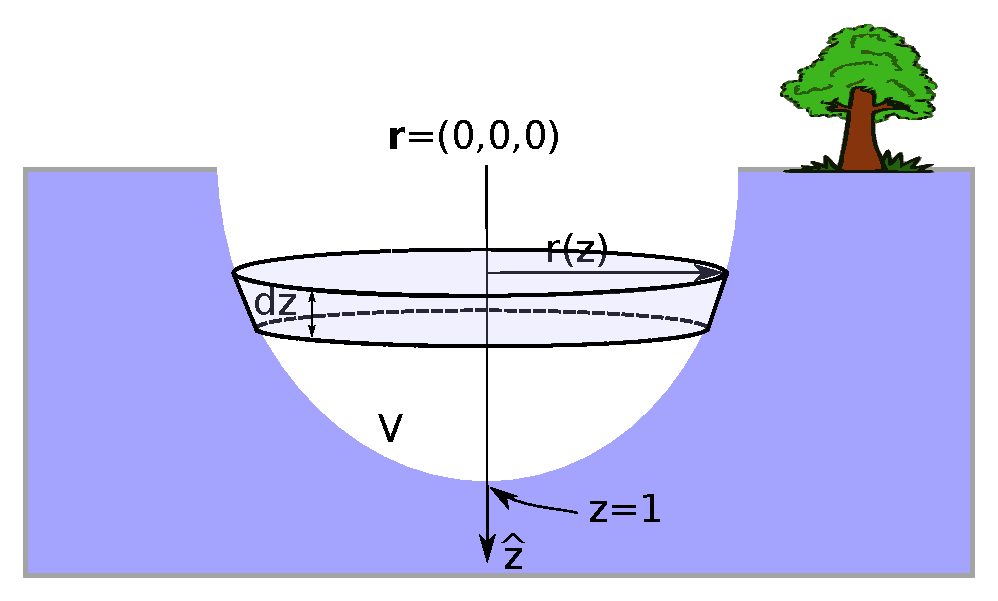
\includegraphics[width=\columnwidth]{crater1}
  \caption{This hemisphere depicts an impact crater of unit
    radius. One way to represent the volume $V$ is to consider discs
    of thickness $dz$ and radius $r(z)$, as drawn.}
  \label{fig:crater}
\end{figure}

This allows us to compute the left-hand side of
equation~\ref{eq:conservenergy}, {\it as if} all the mass $m_c$ was at
one point that is an average of the location of all points in the
hemisphere. This coordinate $\mathbf{R}$ is called the {\it centre of
  mass}. If we divide the hemisphere in $n$ small masses $m_i$ at
location $r_i$ ($i=1,n$), then
\begin{equation}
  \sum _{i=1}^{n}m_{i}(\mathbf {r} _{i}-\mathbf {R} )=0.
  \label{eq:discretecentreofmass}
\end{equation}
In the limit that $n$ goes to infinity, we get the integral version:
\begin{equation} 
  \iiint \limits _{V}\rho (\mathbf {r} )(\mathbf {r} -\mathbf {R} )dV=0.
  \label{eq:integralcentreofmass}
\end{equation}
Because we assume a constant density for our crater material, the
centre of mass $\mathbf{R}$ is equal to the {\it centroid}.

\begin{questions}
  \question[10] Show that
  equation~\ref{eq:integralcentreofmass} reduces to
  \begin{equation} 
    \mathbf{R} = \frac{1}{V}\iiint \limits _{V}\mathbf{r}dV.
    \label{eq:integralcentroid}
  \end{equation}
  \begin{solutionorlines}[3.5in]
    \begin{align*} 
      \iiint \limits _{V}\rho (\mathbf {r} )(\mathbf {r} -\mathbf {R} )dV=0\\
      \rho \left(\iiint \limits _{V}\mathbf {r}dV - \iiint \limits _{V}
      \mathbf {R}dV \right) =0\\
      \rho \iiint \limits _{V}\mathbf {r}dV = \mathbf{R}M\\
      \mathbf{R} = \frac{1}{V}\iiint \limits _{V}\mathbf{r}dV.
    \end{align*}
  \end{solutionorlines}
  In Figure~\ref{fig:crater}, we use a cylindrical coordinate
  system. The vertical coordinate is $z$, a radial $r$, and an unlabeled
  angle around the z-axis $\phi$.  
  
  \question[10] Explain why we can
  reduce the general -- three-dimensional -- coordinate
  $\mathbf{r}=z\hat{\mathbf{z}}$, in this case, so that
  \begin{equation} 
    \mathbf{R} = \frac{1}{V}\iiint \limits _{V}z\hat{\mathbf{z}}dV.
    \label{eq:centroidinz}
  \end{equation}
  \begin{solutionorlines}[2in]
    The centre of mass is along the z-axis for this symmetric body with
    a constant density.
  \end{solutionorlines}
  
  Next, we are going to define these infinitesimal volumes and sum over
  all that make up the hemisphere. The elementary volume $dV$ can be
  taken as a horizontal disk with thickness $dz$, as drawn in
  Figure~\ref{fig:crater}. \question[10] Show that
  $dV= \pi \left(1-z^2\right)dz$.
  \begin{solutionorlines}[2in]
    The area of the disc is $\pi r^2$, and Pythagoras theorem says that
    $r^2 = 1-z^2$. With a disc thickness of $dz$, this all combines to
    $dV= \pi \left(1-z^2\right)dz$.
  \end{solutionorlines}
  \question[10] Integrate over $V$ by integrating over all horizontal
  disks $dV$ between $z=0$ to $z=1$, to determine the centre of mass of
  the material displaced by the crater.
  \begin{solutionorlines}[2.5in]
    \begin{align*} 
      \mathbf{R} = \frac{1}{V}\iiint \limits _{V}z\hat{\mathbf{z}}dV\\
      \mathbf{R} = \frac{\hat{\mathbf{z}}\pi}{V}\int \limits _{0}^1 z 
      \left(1-z^2\right)dz\\
      \mathbf{R} = \frac{\hat{\mathbf{z}}\pi}{2\pi 1^3/3}\left[z^2/2-z^4/4
      \right]_0^1\\
      \mathbf{R} = \frac{\hat{\mathbf{z}}}{2/3}/4\\
      \mathbf{R} = 3\hat{\mathbf{z}}/8    
    \end{align*}
  \end{solutionorlines}
  \question[10] Draw the centre of mass $\mathbf{R}$ in
  Figure~\ref{fig:crater}, and explain why this position makes sense to
  you. Comment on the horizontal and the vertical component of
  $\mathbf{R}$.
  \begin{solutionorlines}[2in]
    symmetry arguments place the centre of mass on the z-axis. Because
    there is more mass near the surface (where the crater is wider),
    we'd expect the centre of mass to be above $z=1/2$.
  \end{solutionorlines}
  
  \subsection{Craters of the Moon}
  \label{sec:moon}
  
  The following investigation allows you to explore the nature of the
  craters that can be easily seen on the surface of the Moon and to
  speculate what a similar bombardment of the Earth would have done to
  it.

  \question[10] Select sector F4 on
  {\color{blue} \url{https://fullmoonatlas.com/atlas/}}. Using the information at the top of the
  page, identify the names and locations of at least two of the craters in the image. Find out their diameters and write these below.
   \begin{solutionorlines}[1in]
 	Some of the named craters are Purbach (118 km, centre left edge), Arzachel (96 km, top left corner), Regiomontanus (126 x 110 km, just below and adjoining Purbach), and Walther (135 km, larger crater lower left hand corner)
 \end{solutionorlines}
 
 
  \question[10] Save the moon image to file, and open
  it using the ImageJ software (search ``ImageJ" in the start
  menu; see {\color{blue} \url{https://imagej.nih.gov/ij/docs/index.html}} for
  documentation and tutorials). Using the straight line tool in ImageJ, measure the diameters (in pixels) of the craters for which you already know the true diameters. What is the pixel size in km? 
  \begin{solutionorlines}[1in]
    Check, but we think 0.78 px/km
  \end{solutionorlines}

  Set the scale using Analyze $\rightarrow$ Set Scale, and
  measure/annotate other craters with the straight line tool. Each
  measurement can be automatically recorded in a spreadsheet by
  pressing ``M''. Save the recorded data with a ``.csv'' extension.

  \question[10] Draw a histogram in Python by importing and plotting
  the estimated crater sizes in the csv file (We use python, because
  {\color{blue} \href{http://www.sciencemag.org/news/2016/08/one-five-genetics-papers-contains-errors-thanks-microsoft-excel}{\textsc{Excel
      is not for scientists}}}!). See the {\color{blue} \href{https://pandas.pydata.org/docs/reference/api/pandas.read_csv.html}{pandas documentation}} for help with importing csv files, and
  {\color{blue} \url{https://matplotlib.org/1.2.1/examples/pylab_examples/histogram_demo.html}} for an example of plotting histograms. Attach your annotated map and
  histogram of your estimated crater sizes to this report.
\pagebreak
  \question[10] What do you infer from this distribution?
  \begin{solutionorlines}[2in]
    More small than large craters, and small ones come often after large
    (of course, large late craters would wipe out small crater evidence)
  \end{solutionorlines}
  \question[10] Derive a formula, based on what you learned in the
  lectures, relating the diameter of the asteroid that produced the
  crater to the diameter of the crater. List your assumptions and
  {\bf re-label the crater size axis of your original histogram with the
  approximate asteroid diameter.}
  \begin{solutionorlines}[6in]
    Starting with equation~\ref{eq:conservenergy}, and taking the steps
    defined in lecture 2 of GEOPHYS213, we get
    $r_a = \left(r_c^3 g h /v_a^2\right)^{1/3}$. $h=3r_c/8$, and we
    assumed that the density of the lunar surface material is constant
    and equal to the density of the asteroid. The gravitational
    acceleration on the moon is $g=1.6$m/s$^2$, so that:
    $r_a = \left(0.6r_c^4/v_a^2\right)^{1/3}$.
  \end{solutionorlines}
  
  \question[10] Study sector E2 of the Moon, next. How do you account
  for the great differences between this sector and F4? 
  \begin{solutionorlines}[2in]
    E2 has many fewer craters. It is a Mare, composed of dark basalts,
    roughly 3.5 GA old. F4 is highlands, around 4 GA old. As E2 has
    fewer craters, much of the asteroid action may have been early on in the
    formation of the moon.
  \end{solutionorlines}
  The gravitational acceleration of $g$ at the surface is different on
  the Moon than the Earth. \question[10] How would you expect a similar
  asteroidal bombardment to have affected the surface of the Earth?  How
  would the presence of the Earth's atmosphere have affected the
  situation on Earth?
  \begin{solutionorlines}[2in]
    a smaller $g$ on the Moon, means that lunar craters are larger than
    on the Earth, for the same size asteroid (see
    equation~\ref{eq:conservenergy}, implying a factor of more than 5 in
    radius difference).
  \end{solutionorlines}
\end{questions}
\end{document}
%%% Local Variables:
%%% mode: latex
%%% TeX-master: t
%%% End:
